\section{Extended Examples}
\label{sec:extended_examples}

\subsection{Counting $n$-grams}

In this example, we'll use graph operations to count the number of $n$-grams in
a string.

Suppose we have a string $aaabaa$ and we want to know the frequency of each
bigram. In this case the bigrams contained in the string are $aa$, $ab$, and
$ba$ with frequencies of $3$, $1$, and $1$ respectively. In the general case we
are given an input string and an $n$-gram and the goal is to count the number
of occurrences of the $n$-gram in the input string.

For a given $n$-gram, the first step is to construct the graph which matches
that $n$-gram at any location in the string. If $\vy$ denotes the $n$-gram, we
want to construct the graph equivalent of the regular expression $.*\vy.*$
where $.*$ indicates zero of more occurrences of any token in the token set.

Suppose we want to count the number of ocurrences of the bigram $aa$ in
$aaabaa$. For the bigram $aa$, and the token set $\{a, b, c\}$, the $n$-gram
matching graph is shown in figure~\ref{fig:bigram_aa}. The first and last state
allow self-loops on any token in the token set. These states correspond to the
$.*$ at the beginning and end of the expression $.*\vy.*$.

\begin{figure}
    \centering
    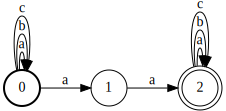
\includegraphics[scale=\dotscale]{figures/bigram_aa}
    \caption{A graph which matches the bigram $aa$.}
    \label{fig:bigram_aa}
\end{figure}

We can encode the string $aaabaa$ with a simple linear graph, as in
figure~\ref{fig:ngram_string}.

\begin{figure}
    \centering
    \includegraphics[scale=\dotscale]{figures/ngram_string}
    \caption{A representation of the sequence $aaabaa$ as a linear graph for
    use in computing the frequency of a given $n$-gram.}
    \label{fig:ngram_string}
\end{figure}

We then compute the intersection of the graph representing the string and the
graph representing the bigram. The intersected graph is in
figure~\ref{fig:bigram_paths}. The number of paths in this graph represents the
number of occurrences of the bigram in the string.

\begin{figure}
    \centering
    \includegraphics[scale=\dotscale]{figures/bigram_paths}
    \caption{The graph represents the intersection of the $n$-gram graph for
    $aa$ with the graph representing $aaabaa$. The number of unique paths in
    this graph, in this case $3$, is the frequency of the $n$-gram $ab$.}
    \label{fig:bigram_paths}
\end{figure}

Since each path has a weight of $0$, we can count the number of unique paths in
the intersected graph by using the forward score. Assume the intersected graph
has $p$ paths. The forward score of the graph is $s = \log \sum_{i=1}^p e^0 =
\log p$. So the total number of paths is $p = e^s$.

\subsection{Edit Distance}

In this example we'll use transducers to compute the Levenshtein edit distance
between two sequences. The edit distance is a way to measure the similarity
between two sequences by computing the minimum number of operations required to
change one sequence into the other. The Levenshtein edit distance allows for
insertion, deletion, and substitution operations.

For example, consider the two strings ``saturday'' and ``sunday''. The edit
distance between them is $3$. One way to minimally edit ``saturday'' to
``sunday'' is with two deletions (\texttt{D}) and a substitution (\texttt{S})
as below:

\begin{center}
\texttt{
    \begin{tabular}{c c c c c c c c}
        s & a & t & u & r & d & a & y \\
          & D & D &   & S &   &   &   \\
        s &   &   & u & n & d & a & y \\
    \end{tabular}
}
\end{center}

We can compute the edit distance between two strings with the use of
transducers. The idea is to transduce the first string into the second
according to the allowed operations encoded as a graph.

We first construct an edits graph $\gE$ which encodes the allowed operations.
An example of an edits graph assuming a token set of $\{a, b\}$ is shown in
figure~\ref{fig:edits}.  The insertion of a token is represented by the arcs
from state $0$ to state $1$ and has a cost of $1$. The deletion of a token is
represented by the arcs from state $0$ to state $2$ which also incur a cost of
$1$. All possible substitutions are encoded in the arcs from $0$ to $3$ and
again have a cost of $1$. We also have to encode the possibility of leaving a
token unchanged. This is represented on the arcs from $0$ to $4$, and the cost
is $0$.

\begin{figure}
    \centering
    \includegraphics[scale=\dotscale]{figures/edits}
    \caption{An example of an edits graph $\gE$ for the token set $\{a, b\}$.
    The graph encodes the allowed edit distance operations and their associated
    penalties.}
    \label{fig:edits}
\end{figure}

We then take closure of the edits graph $\gE$ to represent the fact that we can
make zero or more of any of the allowed edits. We then encode the first
sequence $\vx$ in a graph $\gX$ and the second sequence $\vy$ in a graph $\gY$.
All possible ways of editing $\vx$ to $\vy$ can be computed by taking the
composition:

$$
\gP = \gX \circ \gE^* \circ \gY.
$$

The graph $\gP$ represents the set of all possible unique ways we can edit the
sequence $\vx$ into $\vy$. The score of a given path in $\gP$ is the associated
cost. We can then find the edit distance by computing the path with the
smallest score in $\gP$. For this, we could use the Viterbi algorithm with a
$\min$ instead of a $\max$. Alternatively, we can use weights of $-1$ instead
of $1$ in $\gE$ and use the Viterbi algorithm unchanged. In this case, the path
with the largest score (the one with the least negative score) represents the
edit distance. The actual edits (*i.e.* the insertions, deletions, and
substitutions) can be found by computing the Viterbi path.

\begin{example}
Compute the edit distance graph $\gP$ between $\vx = aba$ and $\vy = aabb$, the
edit distance between the two sequences, and one possible set of operations
which attain the edit distance.
\end{example}

Using an equivalent but more compact representation of the edit distance graph
$\gE^*$ yields the graph $\gP = \gX \circ \gE^* \circ \gY$, shown in
figure~\ref{fig:edit_paths}. Each path in $\gP$ represents a unique conversion
of $\gX$ into $\gY$ using insertion, deletion, and substitution operations. The
negation of the score of the path is the number of such operations required.

For example, the path along the state sequence $0 \rightarrow 1 \rightarrow 6
\rightarrow 11 \rightarrow 16$ converts $\vx$ to $\vy$ with a distance of two
using an insertion at the second letter and a substitution at the end:

\begin{center}
\texttt{
    \begin{tabular}{c c c c}
        a &   & b & a \\
          & I &   & S \\
        a & a & b & b \\
    \end{tabular}
}
\end{center}

\begin{figure}
    \centering
    \includegraphics[scale=0.5]{figures/edit_paths}
    \caption{The graph $\gP = \gX \circ \gE^* \circ \gY$ represents all
    possible ways to convert $\vx = aba$ to $\vy = aabb$ using insertions,
    deletions, and substitutions. Since the penalties are negative, the score
    of the highest scoring path is the edit distance between the two sequences.
    The path itself encodes the sequence of operations required.}
    \label{fig:edit_paths}
\end{figure}

The Viterbi score and Viterbi path yield the edit distance between $\vx$ and
$\vy$ and the sequence of edit operations required to attain the edit distance.
The Viterbi path for the example is shown in figure~\ref{fig:edit_path}.

\begin{figure}
    \centering
    \includegraphics[scale=\dotscale]{figures/edit_path}
    \caption{The Viterbi path of the graph $\gP = \gX \circ \gE^* \circ \gY$.
    The edit distance is $2$ with one insertions (the arc between states $0$
    and $1$) and one substitution (the arc between states $3$ and $4$).}
    \label{fig:edit_path}
\end{figure}

\subsection{$n$-gram Language Model}
\label{sec:ngram_model}

In this example we will encode an $n$-gram language model as an acceptor. We
will then use the acceptor to compute the language model probability for a
given sequence.

Let's start with a very simple example. Suppose we have the token set $\{a, b,
c\}$ and we want to construct a unigram langauge model. Given counts of
occurrences for each token in the vocabulary, we can construct an acceptor to
represent the unigram language model. Suppose we are given the probabilities
$0.5$, $0.2$, and $0.3$ for $a$, $b$, and $c$ respectively. The corresponding
unigram graph is shown below. Note that the edge weights are log probabilities.

\begin{figure}
    \centering
    \includegraphics[scale=\dotscale]{figures/unigram}
    \caption{A unigram graph $\gU$ for $\{a, b, c\}$.}
    \label{fig:unigram}
\end{figure}

Now assume we are given the sequence $aa$ for which we would like to compute
the probability. The probability under the language model is $\frac{1}{2} \cdot
\frac{1}{2} = \frac{1}{4}$. We can compute the log probability of $aa$ by
intersecting its graph representation $\gX$ with the unigram graph $\gU$ and
then computing the forward score:

$$
\log p(aa) = \LSE (\gX \circ \gU)
$$


The graph below shows the intersection $\gX \circ \gU$. The arc edges in the
intersected graph contain the correct unigram scores, and the forward score
gives the log probability of the sequence $aa$. In this case, the Viterbi score
would give the same result since the graph has only one path.

\begin{figure}
    \centering
    \includegraphics[scale=\dotscale]{figures/unigram_aa_scored}
    \caption{The sequence $aa$ scored with the unigram log probabilities from
    the graph $\gU$ above.}
    \label{fig:unigram_aa_scored}
\end{figure}

For an arbitrary sequence $\vx$ with a graph representation $\gX$ and an
arbitrary $n$-gram language model with graph representation $\gN$, the log
probability of $\vx$ is given by:

$$
\log p(\vx) = \LSE(\gX \circ \gN).
$$

Next, let's see how to represent a bigram language model as a graph. From
there, the generalization to arbitrary order $n$ is relatively straightforward.
Assume again we have the token set $\{a, b, c\}$. The bigram model is shown in
the graph below.

\begin{figure}
    \centering
    \includegraphics[scale=\dotscale]{figures/bigram}
    \caption{A bigram model for the token set $\{a, b, c\}$. Each arc is
    labeled with the next observed token and the corresponding bigram
    probability.}
    \label{fig:bigram}
\end{figure}

Each state is labeled with the token representing the most recently seen input.
For a bigram model we only need to remember the previous token to know which
score to use when processing the next token. For a trigram model we would need
to remember the previous two tokens. For an $n$-gram model we would need to
remember the previous $n-1$ tokens. The label and score pair leaving each state
represent the corresponding conditional probability (technically these should
be log probabilities). Each state has an outgoing arc for every possible token
in the token set.

\begin{example}
\label{ex:ngram}
Compute the number of states and arcs in a graph representation of an $n$-gram
language model for a given order $n$ and a token set size of $v$.
\end{example}

\begin{proof}[\unskip\nopunct]
For order $n$, the graph needs a state for every possible token sequence of
length $n-1$. This means that the graph will have $v^{n-1}$ states. Each state
has $v$ outgoing arcs. Thus the total number of arcs in the graph is $v \cdot
v^{n-1}= v^n$. This should be expected given that the language model assigns a
score for every possible sequence of length $n$.
\end{proof}

\subsection{Automatic Segmentation Criterion}

In machine-learning applications with sequential data, we often need to compute
a conditional probability of an output sequence given an input sequence when
the two sequences do not have the same length. The Automatic Segmentation
criterion (ASG) is one of several common loss functions for which this is
possible. However, ASG is limited to the case when the output sequence is no
longer than the input sequence.

Assume we have an input sequence of $T$ vectors $\mX = [\vx_1, \ldots, \vx_T]$
and an output sequence of $U$ tokens, $\vy = [y_1, \ldots, y_U]$ such that $U
\le T$. We don't know the actual alignment between $\mX$ and $\vy$, and in many
applications we don't need it. For example, in speech recognition $\mX$
consists of frames of Fourier-transformed audio, and $\vy$ could be letters of
a transcript. We usually don't need to know how $\vy$ aligns to $\mX$; we only
require that $\vy$ is the correct transcript. To get around not knowing this
alignment, the ASG criterion marginalizes over all possible alignments between
$\mX$ and $\vy$.

In ASG, the output sequence is aligned to a given input by allowing one or more
consecutive repeats of each token in the output. Suppose we have an input of
length $5$ and the output sequence $ab$. Some possible alignments of the output
are $aaabb$, $abbbb$, and $aaaab$. Some invalid alignmets are $abbbba$, $aaab$,
and $aaaaa$. These are invalid because the first corresponds to the output
$aba$, the second is too short, and the third corresponds to the output $a$.

For each time-step of the input, we have a model $s_t(a)$ which assigns a score
for every possible output token $a$. Note the model $s_t(\cdot)$ is conditioned
on some or all of $\mX$, but I won't inlcude this in the notation for
simplicity. Let $\va = [a_1, \ldots, a_T]$ be one possible aligment between
$\mX$ and $\vy$. The alignment $\va$ also has length $T$. To compute a score
for $\va$, we sum the sequence of scores for each token:

$$
s(\va) = \sum_{t=1}^T s_t(a_t)
$$

Let $\gA_{\mX,\vy}$ denote the set of all possible alignments between $\mX$ and
$\vy$. We use the individual alignment scores to compute a conditional
probability of the output $\vy$ given the input $\mX$ by marginalizing over
$\gA_{\mX,\vy}$:

$$
\log p(\vy \mid \mX) = \LSE_{\va \in \gA_{\mX, \vy}} s(\va) - \log Z.
$$

The normalization term $Z$ is given by:

$$
Z = \sum_{\va \in \gZ_\mX} e^{s(\va)},
$$

where $\gZ_\mX$ is the set of all possible length $T$ alignments (the same
length as $X$). Computing the summations over $\gA_{\mX,\vy}$ and $\gZ_\mX$
explicitly is not tractable because the sizes of these sets grow rapidly with
the lengths of $\mX$ and $\vy$. Let's instead use automata to encode these sets
and efficiently compute the summation using the forward score operation. I will
use the script variables $\gA_{\mX,\vy}$ and $\gZ_\mX$ to represent both sets
of sequences and the analogous graph. It will be clear from context which
representation is intended.

Let's start with the normalization term $Z$. The set $\gZ_\mX$ encodes all
possible outputs of length $T$, where $T$ is the length of $\mX$. As an
example, assume $T=4$ and we have three possible output tokens $\{a, b, c\}$.
If the scores for each otuput are independent, we can represent $\gZ_\mX$ with
the graph below. The scores on the arcs are given by the model $s_t(\cdot)$.
These scores are often called the *emissions*, and the graph itself is
sometimes called the emissions graph. I'll use $\gE$ to represent the emissions
graph. In this case the emissions graph $\gE$ is the same as the normalization
graph $\gZ_\mX$; however, in general they may be different. The log
normalization term is the forward score of the emissions graph, $\log Z =
\LSE(\gE)$.

\begin{figure}
    \centering
    \includegraphics[scale=\dotscale]{figures/asg_emissions}
    \caption{An emissions graph $\gE$ with $T=4$ time-steps and a token set of
    $\{a, b, c\}$.}
    \label{fig:asg_emissions}
\end{figure}

Let's turn to the set $\gA_{\mX, \vy}$ which we will also represent as an
acceptor. This acceptor should have a path for every possible alignment between
$\mX$ and $\vy$. We'll construct $\gA_{\mX, \vy}$ in two steps. First, we can
encode the set of allowed alignments of arbitrary length for a given sequence
$\vy$ with a graph, $\gA_\vy$. As an example, for the sequence $ab$ the graph
$\gA_\vy$ is shown below.

\begin{figure}
    \centering
    \includegraphics[scale=\dotscale]{figures/asg_alignments}
    \caption{The ASG alignment graph $\gA_\vy$ for the sequence $ab$. The graph
    encodes the fact that each output token can repeat one or more times in an
    arbitrary length alignment.}
    \label{fig:asg_alignments}
\end{figure}

This graph has a simple interpretation. Each token in the output $ab$ can
repeat one or more times in the alignment. We can then construct
$\gA_{\mX,\vy}$ by intersecting $\gA_\vy$ with the emissions graph $\gE$, which
represents all possible sequences of length $T$. This gives $\gA_{\mX,\vy} =
\gA_\vy \circ \gE$. An example of $\gA_{\mX, \vy}$ is shown below for the
sequence $ab$ with $T=4$.

\begin{figure}
    \centering
    \includegraphics[scale=\dotscale]{figures/asg_constrained}
    \caption{The alignment graph $\gA_{\mX, \vy}$ for the an input $\mX$ with
    $T=4$ time-steps and an output $\vy = ab$.}
    \label{fig:asg_constrained}
\end{figure}

In terms of graph operations, we can write the ASG criterion as:

$$
p(\vy \mid \mX) = \LSE(\gA_\vy \circ \gE) - \LSE(\gE).
$$

%% TODO
Aside: Global or Local Normalization

The equation for the ASG criterion is *globally normalized*. The term $Z$ is
the global normalization term and it ensure that the conditional probability
$p(\vy \mid \mX)$ is a valid distribution; that is it sums to one over $\vy$.
The global normalization term $Z$ (also known as the partition function) is
often the most expensive part of the loss to compute.

In some cases the global normalization can be avoided by using a *local
normalization*. For example, in the version of ASG presented above, the path
score for $\va$ decomposes into a separate score for each time-step. In this
case, we can compute the exact some loss by normalizing the scores $s_t(y)$ at
each time-step and dropping the global normalizer $Z$. Concretely, we compute
the normalized scores at each time-step:

$$
p_t(y) = \frac{e^{s_t(y)}}{\sum_z e^{s_t(z)}}.
$$

We then replace the unnormalized scores with the log-normalized scores when
computing the score for an alignment:

$$
\log p(\va) = \sum_{t=1}^T \log p_t(a_t)
$$

As a last step, we remove the global normalization term $Z$ from the loss
function, but leave it otherwise unchanged:

$$
\log p(\vy \mid \mX) = \LSE_{\va \in \gA_{\mX, \vy}} \log p(\va)
$$

In the version which uses graph operations, we use the log-normalized scores
$\log p_t(y)$ for the arc weights on the emissions graph $\gE$. The graph based
loss function then simplifies to:

$$
\log p(\vy \mid \mX) = \LSE(\gA_\vy \circ \gE)
$$

We can prove that this locally normalized version of the ASG loss is equivalent
to the globally normalized version. To do this, we need to show that:

$$
\LSE_{\va \in \gA_{\mX, \vy}} \log p(\va) = \LSE_{\va \in \gA_{\mX, \vy}} s(\va) - \log Z
$$

To prove this we'll need to rely on two identities. The first identity is:

$$
\LSE_x( x + y) = \LSE(x) + y
$$

which we can prove:

$$
\LSE_x (x + y) = \log \sum_x e^{x+y} = \log \sum_x e^x e^y = \log \sum_x e^x + \log e^y = \LSE(x) + y.
$$

The second identity let's us rearrange products and sums:

$$
\prod_{t=1}^T \sum_{z} s_t(z) = \sum_\vz \prod_{t=1}^t s_t(z_t).
$$

In words, the product over $t$ of the sum over possible values of the token $z$
is the same as the sum over all possible token sequences $\vz$ of length $T$ of
the product over each time-step in the sequence. A short proof is below:

\begin{align*}
\prod_{t=1}^T \sum_{z} s_t(z) &= \left(\sum_{z} s_1(z)\right) \ldots \left(\sum_{z} s_T(z)\right) \\
&= \sum_{z_1} \ldots \sum_{z_T} \prod_{t=1}^t s_t(z_t) \\
&= \sum_{\vz}\prod_{t=1}^t s_t(z_t).
\end{align*}

Starting from the left hand side of the equation we are trying to show, we have:

\begin{align*}
\LSE_{\va \in \gA_{\mX, \vy}} \log p(\va) &= \LSE_{\va \in \gA_{\mX, \vy}} \sum_{t=1}^T \log p_t(a_t) \\
&= \LSE_{\va \in \gA_{\mX, \vy}} \sum_{t=1}^T \log \frac{e^{s_t(a_t)}}{\sum_z e^{s_t(z)}} \\
&= \LSE_{\va \in \gA_{\mX, \vy}} \left( \sum_{t=1}^T s_t(a_t) - \sum_{t=1}^T \log \sum_z e^{s_t(z)} \right)\\
\end{align*}

Using the first identity, we get:

\begin{align*}
\LSE_{\va \in \gA_{\mX, \vy}} \log p(\va) &= \LSE_{\va \in \gA_{\mX, \vy}} \left( \sum_{t=1}^T s_t(a_t)\right) - \sum_{t=1}^T \log \sum_z e^{s_t(z)} \\
\end{align*}

The first term on the right is:

$$
\LSE_{\va \in \gA_{\mX, \vy}} \left( \sum_{t=1}^T s_t(a_t)\right) = \LSE_{\va \in \gA_{\mX, \vy}} s(\va),
$$

Using the second idenity, the second term on the right becomes:

\begin{align*}
\sum_{t=1}^T \log \sum_z e^{s_t(z)} &= \log \prod_{t=1}^T \sum_z e^{s_t(z)} \\
&= \log \sum_{\vz \in \mathcal{\gZ_\mX}} \prod_{t=1}^T e^{s_t(z_t)} \\
&= \log \sum_{\vz \in \mathcal{\gZ_\mX}} e^{\sum_{t=1}^T s_t(z_t)} \\
&= \log \sum_{\vz \in \mathcal{\gZ_\mX}} e^{s(\vz)} \\
&= \log Z.
\end{align*}

Putting these two terms together yields the right hand side of what we wanted to show.

%%% END ASIDE

\subsubsection{Transitions}

The original ASG loss function also includes bigram transition scores. The
alignment score with transitions, $h(a_{t-1}, a_t)$, included is given by:

$$
s(\va) = \sum_{t=1}^T s_t(a_t) + h(a_t, a_{t-1}),
$$

where $a_0$ is a special start of sequence token $\textrm{<s>}$. We can use the
alignment scores in the same manner as above and the rest of the loss function
is unchanged.

Let's see how to incorporate transitions using an acceptor and graph
operations. I'll rely on the ideas introduced in section~\ref{sec:ngram_model}
on $n$-gram langauge models, so now is a good time to review that section. The
first step is to encode the bigram model as a graph, as shown below:

\begin{figure}
    \centering
    \includegraphics[scale=\dotscale]{figures/asg_bigrams}
    \caption{The acceptor represents a bigram transition model for the token
    set $\{a, b, c\}$ (the arc weights are not shown). Each path begins in the
    start state denoted by the start-of-sequence symbol $\sos$.}
    \label{fig:asg_bigrams}
\end{figure}

To incorporate transition scores for the output sequence, we intersect the
bigram graph $\gB$ with the output alignment graph $\gA_\vy$. To incorporate
transition scores in the normalization term $Z$, we intersect $\gB$ with the
emissions graph $\gE$. The loss function using graph operations including
transitions becomes:

$$
p(\vy \mid \mX) = \LSE(\gB \circ \gA_\vy \circ \gE) - \LSE(\gB \circ \gE).
$$

We see here an example of the expressive power of a graph-based implementation
of the loss function. In a non-graph based implementation of ASG, the use of a
bigram transition function is hard-coded. In the graph-based version, the
transition model $\gB$ could be a unigram, bigram, trigram, or otherwise
arbitrary $n$-gram. Of course, the size of the transition graph increases
rapidly with the order $n$ and the size of the token set (see
example~\ref{ex:ngram}). This causes problems with both sample and
computational efficiency. Thus, in practice ASG is used with a bigram
transition model and token set sizes rarely larger than a hundred.

The arc weights on the transition graph (the scores $h(a_t, a_{t-1})$), are
typically parameters of the model and learned directly. This means we need to
compute the gradient of the ASG loss with respect to these scores. These
derivatives are straightforward to compute in a framework with automatic
differentiation.

A complete implementation of the ASG loss function which takes as input an
emissions graph $\gE$, a transitions graph $\gB$, and an output alignment graph
$\gA_\vy$ is shown below. I would like to make three observations about this
code:

\begin{enumerate}
    \item The implementation is concise. Given the appropriate graph inputs,
        the complete loss function requires only eight short lines using ten
        function calls.

    \item The code should look familiar to users of tensor-based frameworks
        like PyTorch. Other than the different operation names, the imperative
        style and gradient computation is no different with graphs than it is
        with tensors.

    \item The code is generic. For example, we can pass a trigram model as the
        input graph argument `B` without needing to change the function.
\end{enumerate}


%```python
%def ASG(E, B, AY):
%    # Compute constrained and normalization graphs:
%    AXY = gtn.intersect(gtn.intersect(B, AY), E)
%    ZX = gtn.intersect(B, E)
%
%    # Forward both graphs:
%    AXY_score = gtn.forward_score(AXY)
%    ZX_score = gtn.forward_score(ZX)
%
%    # Compute the loss:
%    loss = gtn.negate(gtn.subtract(AXY_score, ZX_score))
%
%    # Clear the previous gradients:
%    E.zero_grad()
%    B.zero_grad()
%
%    # Compute gradients:
%    gtn.backward(loss, retain_graph=False)
%
%    return loss.item()

\subsubsection{ASG with Transducers}

As a final step, I'll show how to construct the ASG criterion from even simpler
transducer buildling blocks. The advantage of this approach is that it lets us
easily experiment with changes to the criterion at a deeper level.

Our goal is to compute $\gA_\vy$ from simpler graphs instead of hard-coding its
structure directly. The simpler graphs will represent the individual tokens and
the target sequence $\vy$.

The target sequence graph $\gY$ is a simple linear-chain graph with arc labels
taken consecutively from the sequence $\vy$. The graph below shows an example
for the sequence $ab$.

\begin{figure}
    \centering
    \includegraphics[scale=\dotscale]{figures/asg_target_ab}
    \caption{The graph $\gY$ corresponding to the target sequence $\vy = ab$.}
    \label{fig:asg_target_ab}
\end{figure}

Next we construct the individual token graphs. These graphs encode the
assumption that each token in an output maps to one or more repeats of the same
token in an alignment. For example for the output $\vy = ab$ and alignment $\va
= aaaabb$ the token $a$ maps to $aaaa$ and $b$ maps to  $bb$. For the token
$a$, we can construct the token graph $\gT_a$ shown below which has the desired
property.

\begin{figure}
    \centering
    \includegraphics[scale=\dotscale]{figures/asg_tokens_a}
    \caption{An individual token graph $\gT_a$ for the token $a$. The graph
    encodes the fact that the output $a$ can map to one or more repeats in the
    alignment.}
    \label{fig:asg_tokens_a}
\end{figure}

Since an output sequence can consist of any sequence of tokens from the token
set, we construct the complete token graph $\gT$ by taking the union of the
individual token graphs and computing the closure. If we have a token set $\{a,
b, c\}$, then we construct individual token graphs $\gT_a$, $\gT_b$, and
$\gT_c$. The complete token graph $\gT$ is given by $\gT = (\gT_a + \gT_b +
\gT_c)^*$.

\begin{figure}
    \centering
    \includegraphics[scale=\dotscale]{figures/asg_tokens}
    \caption{The complete token graph $\gT$ for the token set $\{a, b, c\}$.
    The token graph is constructed by taking the closure of the union of the
    individual token graphs, $\gT = \gT_a + \gT_b + \gT_c$.}
    \label{fig:asg_tokens}
\end{figure}

The graph $\gA_\vy$ can then be constructed by composing $\gT$ and $\gY$. In
other words, $\gA_\vy = \gT \circ \gY$. We have to be careful here. The graphs
$\gT$ and $\gY$ are transducers and their order in the composition makes a
difference. Because of the way we constructed them, we will only get the
correct $\gA_\vy$ if $\gT$ is on the first argument to the composition.

At this point, we can compute the ASG loss just as before. The remaining graphs
$\gE$ and $\gB$ are unchanged.

As we mentioned, this decomposition of the ASG loss using simple graph building
blokcs makes it easier to change. In the following section, we will show how to
construct a different algorithm, Connectionist Temporal Classification, with
only a minor modification to the ASG loss.

\subsection{Connectionist Temporal Classification}

Connectionist Temporal Classification (CTC) is another loss function which
assigns a conditional probability $p(\vy \mid \mX)$ when the input length $T$
and output length $U$ are variable, and the alignment between them is unknown.
Like ASG, CTC gets around the fact that the alignment is unknown by assuming a
set of allowed alignments and marginilazing over this set. In CTC, the length
of the output $\vy$ is also constrained in terms of the length of the input.
For CTC, the output length $U$ must satisfy $U + R_\vy \le T$, where $R_\vy$ is
the number of consecutive repeats in $\vy$.

The ASG loss function has two modeling limitations which CTC attempts to
improve. First, ASG does not elegantly handle repeat tokens in the output.
Second, ASG does not allow for optional null inputs. I'll discuss each of these
in turn.

\paragraph{Repeat Tokens:} A repeat token is two consecutive tokens with the
same value. For example, the $b$'s in $abba$ is a repeat, but the $a$ is not.
In ASG, repeat tokens in the output create an ambiguity. A single alignment can
map to multiple output sequences. For example, consider the alignment $abbbaa$.
This can map to any of the outputs $aba$, $abba$, $abbba$, $abaa$, $abbaa$, or
$abbbaa$. There are several heuristics to resolve this. One option is to use
special tokens for repeat characters. For example if $\vy = abba$, then we
could encode it as $ab_2a$, where $b_2$ corresponds to two $b$'s.In this case,
the alignment $abbba$ corresponds to the output $aba$,the alignment
$ab_2b_2b_2a$ corresponds to the output $abba$, and the alignment $abbb_2$
corresponds to $abbba$.

There are two problems with this solution. First, we have to hard code into the
token set an upper limit on the number of repeats to allow. Second, if we allow
$n$ repeats, then we multiply the token set size by a factor of $n$ causing
potential computation and sample efficiency issues.

\paragraph{Blank Inputs:} The second problem with ASG is it dos not allow
optional null inputs. Any output token $y_u$ must map to a corresponding input
$\vx_t$. In some cases, the $y_u$ may not meaningfully correspond to any input.
The blank token in CTC allows for this by representing an input time step which
does not correspond to any output.

I'll denote the CTC blank token with $\blank$. The token $\blank$ can appear
zero or more times in the alignment, and it can be at the beginning, inbetween,
or end of the tokens of the output $\vy$. If $\vy$ has consecutive repeats,
then there must be at least one $\blank$ between them in any alignment. So the
optional blank token is a solution to both the modeling of null input time
steps as well as repeat tokens in the output. Note also that non-optional blank
between repeat tokens is why in CTC the output length must satisfy $U + R_\vy <
T$.

As an example, suppose we have an input of length $5$ and the output sequence
$abb$. Some allowed alignments are $abb \blank b$, $ab \blank bb$, or $aa b
\blank b$. Some alignments which are not allowed are $aabbb$ and $aa\blank b
b$, both of which correspond to the output $ab$ instead of $abb$.

In equations, CTC is indistinguishable from ASG without transitions. The loss
is given by:

$$
\log p(\vy \mid \mX) = \LSE_{\va \in \gA_{\mX, \vy}} \log p(\va).
$$

The distinction between ASG and CTC is in the set of allowed alignments
$\gA_{\mX, \vy}$.

Assuming we have log normalized scores on the arc weights of the emissions
graph $\gE$, the graph based CTC loss is:

$$
\log p(\vy \mid \mX) = \LSE(\gA_\vy \circ \gE),
$$

where the distinction from ASG is in the graph $\gA_\vy$. An example alignment
graph $\gA_\vy$ for CTC for the sequence $ab$ is shown below.

\begin{figure}
    \centering
    \includegraphics[scale=\dotscale]{figures/ctc_alignments}
    \caption{The CTC alignment graph $\gA_\vy$ for the sequence $ab$. The graph
    encodes the fact that each output token can repeat one or more with an
    optional $\blank$ at the beginning, end, or inbetween $a$ and $b$.}
    \label{fig:ctc_alignments}
\end{figure}

The CTC alignment graph above encodes the assumptions regarding the blank
token, $\blank$. The alignment can optionally start with $\blank$ as in state
$0$. The alignment can optionally end in $\blank$ since both state $3$ and $4$
are accept states. And lastly, the blank is optional between $a$ and $b$ since
there is both an arc between states $1$ and $3$ and a path through state $2$
which emits a $\blank$.

\begin{example}
Construct the CTC $\gA_\vy$ graph for the sequence $aa$.
\end{example}

\begin{proof}[\unskip\nopunct]

\begin{figure}
    \centering
    \includegraphics[scale=\dotscale]{figures/ctc_alignments_aa}
    \caption{The CTC alignment graph $\gA_\vy$ for the sequence $aa$.}
    \label{fig:ctc_alignments_aa}
\end{figure}

The graph $\gA_\vy$ for the sequence $\vy = aa$ is shown above. Notice the
$\blank$ token inbetween the first and second $a$ is not optional. The
onlydifference between the graph for $aa$ and the graph for $ab$ is the removal
of the arc between states $1$ and $3$.
\end{proof}

\subsubsection{CTC from Transducers}

Like ASG we can construct the graph $\gA_\vy$ used in CTC from smaller building
blocks. In fact, one of the motivations of decomposing ASG into simpler
transducer buildling blocks is that it makes constructing CTC almost trivial.
To get CTC, we just need to add the $\blank$ token to the tokens graph with the
correct semantics. The $\blank$ token graph is a single start and accept
state which encodes the fact that the blank is optional. The state has a
self-loop which transduces $\blank$ to $\epsilon$ since $\blank$ never yields
an output token.

In graph operations, for ASG with the alphabet $\{a, b, c\}$, the graph
$\gA_\vy$ is given by:

$$
\gA_\vy = (\gT_a + \gT_b + \gT_c)^* \circ \gY.
$$

Assuming $\gT_\blank$ represents the $\blank$ token transducer as described
above, the CTC graph $\gA_\vy$ is given by:

$$
\gA_\vy = (\gT_a + \gT_b + \gT_c + \gT_\blank)^* \circ \gY.
$$

The equation above shows how CTC is really the result of one core additional
building block encoding the correct behavior of the $\blank$ token. There is
one caveat which is that the equation does not force the $\blank$ token
inbetween repeats, so they are not handled correctly. Encoding this constraint
through operations on the simpler transducers requires more work but is
certainly doable.
